\documentclass{article}
\renewcommand{\baselinestretch}{1.25}

\usepackage{xeCJK}  % support character

% monokai code
\usepackage{color}
\usepackage{minted}
\usemintedstyle{manni}
\setminted{
    linenos,
    fontsize=\footnotesize,
    resetmargins
}

% insert images
\usepackage{graphicx}
\graphicspath{{images/}{../images/}}
\usepackage{amsmath}
\usepackage{caption}
\numberwithin{figure}{section}
\numberwithin{table}{section}
\numberwithin{listing}{section}
\numberwithin{equation}{section}

\usepackage{subcaption}

% hyperlink
\usepackage{hyperref}
\usepackage{xcolor}
\hypersetup{
    colorlinks,
    linkcolor={red!50!black},
    citecolor={blue!50!black},
    urlcolor={blue!80!black}
}

% auto newline in table
\newcommand{\tabincell}[2]{\begin{tabular}{@{}#1@{}}#2\end{tabular}}
\usepackage{multirow}

\usepackage{mathtools}
\usepackage{amsfonts}

\author{郭一隆(2013011189)}
\title{连连看实验报告}

\begin{document}
    \maketitle

    \tableofcontents
    \newpage

    \listoffigures
    \listoftables
    \renewcommand\listoflistingscaption{List of Source Codes}
    \listoflistings
    \newpage

    \section{原创性} % (fold)
    \label{sec:原创性}
        
        \textbf{本次连连看大作业由本人独立思考完成,如有雷同,纯属巧合。}

    % section 原创性 (end)

    \section{制作自己的连连看} % (fold)
    \label{sec:制作自己的连连看}
    
        \begin{enumerate}
            \item 在\texttt{MATLAB}环境下,设置当前路径为\texttt{linkgame},运行\texttt{linkgame}(打开\href{../linkgame/linkgame.fig}{\texttt{linkgame.fig}}或右键\href{../linkgame/linkgame.p}{\texttt{linkgame.p}}点“运行”),熟悉游戏。

                \begin{figure}[H]
                    \centering
                    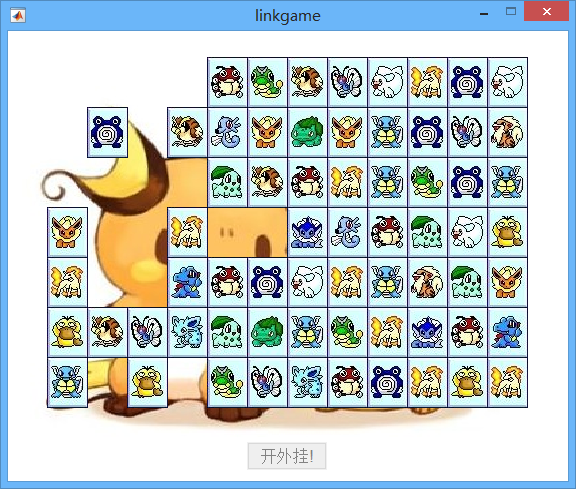
\includegraphics[width=0.7\textwidth]{run_linkgame}
                    \caption{运行连连看}
                \end{figure}

            \item 注意\texttt{linkgame}目录下有个\texttt{detect.p},它的功能时检测块是否可以消除。现将其删掉,然后把\texttt{linkgame\textbackslash reference}目录下的\href{../linkgame/reference/detect.m}{\texttt{detect.m}}复制到\texttt{linkgame}目录下。\href{../linkgame/detect.m}{\texttt{detect.m}}文件中是\texttt{detect}函数,函数以图像块的索引矩阵与要判断的两个块的下标为输入,如果两个块能消掉则输出\texttt{1},否则输出\texttt{0}。根据文件中的注释提示,实现判断块是否可以消除的功能。写完后再次运行\texttt{linkgame},检验游戏是否仍然可以正确运行。

                算法实现分为以下几个步骤:

                \begin{enumerate}
                    \item \textbf{画十字\texttt{adjcross}}:在给定点周围空白处画十字,遇到块则停止。

                        \begin{listing}[H]
                            \inputminted[firstline=29, lastline=48]{matlab}{../linkgame/canlink.m}
                            \caption{\texttt{canlink.m(adjcross)}}
                        \end{listing}

                    \item \textbf{判断是否可直连\texttt{canlink0}}:先判断横纵坐标是否在同一直线,再确认路径上是否有障碍。

                        \begin{listing}[H]
                            \inputminted[firstline=51, lastline=62]{matlab}{../linkgame/canlink.m}
                            \caption{\texttt{canlink.m(canlink0)}}
                        \end{listing}

                    \item \textbf{判断是否可用不超过一个直角的连线连接\texttt{canlink1}}:选取两目标点之一作为起点,画十字;对十字上的点进行遍历,检查是否存在可与另一目标点直连的点。

                        \begin{listing}[H]
                            \inputminted[firstline=65, lastline=86]{matlab}{../linkgame/canlink.m}
                            \caption{\texttt{canlink.m(canlink1)}}
                        \end{listing}

                    \item \textbf{判断可连性\texttt{canlink}}:选取两目标点之一作为起点,画十字;对十字上的点进行遍历,检查是否存在可与另一目标用不超过一个直角的连线连接的点。

                        \inputminted[firstline=1, lastline=26]{matlab}{../linkgame/canlink.m}
                        \begingroup
                            \captionof{listing}{\texttt{canlink.m(main)}}
                        \endgroup
                \end{enumerate}

                再次运行\texttt{linkgame},\href{../linkgame/detect.m}{\texttt{detect.m}}功能正常。

                \begin{minted}{matlab}
function bool = detect(mtx, x1, y1, x2, y2)
    
    [m,n] = size(mtx);
    
    % add surrounding zeros
    mtx = [0,zeros(1,n),0;
        zeros(m,1),mtx,zeros(m,1);
        0,zeros(1,n),0];
    
    origin = mtx(x1+1,y1+1);
    target = mtx(x2+1,y2+1);
    
    if origin == target && canlink(mtx,x1+1,y1+1,x2+1,y2+1)
        bool = 1;
    else
        bool = 0;
    end
       
end
                \end{minted}
                \begingroup
                    \captionof{listing}{\texttt{detect.m(main)}}
                \endgroup

                \begin{figure}[H]
                    \centering
                    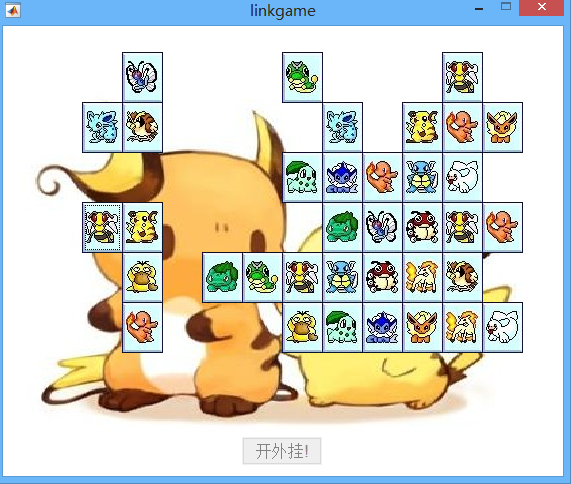
\includegraphics[width=0.7\textwidth]{mydetect_linkgame}
                    \caption{重写\texttt{detect.m}后运行\texttt{linkgame}}
                \end{figure}

            \item “外挂”模式逐一自动消除所有的块的功能是由\texttt{link}目录的\texttt{omg.p}实现的。删掉\texttt{omg.p}重新实现\href{../linkgame/omg.m}{\texttt{omg.m}}。

                根据游戏经验,算法通过以下几个步骤实现:

                \begin{enumerate}
                    \item \textbf{消去相邻的相同块\texttt{matchadj}}:利用自带函数\texttt{diff}实现,注意及时更新原矩阵以及保证多个相同块连续相邻时仍正确工作。

                        \inputminted[firstline=42,lastline=76]{matlab}{../linkgame/omg.m}
                        \begingroup
                            \captionof{listing}{\texttt{omg.m(matchadj)}}
                        \endgroup

                        \begin{figure}[H]
                            \centering
                            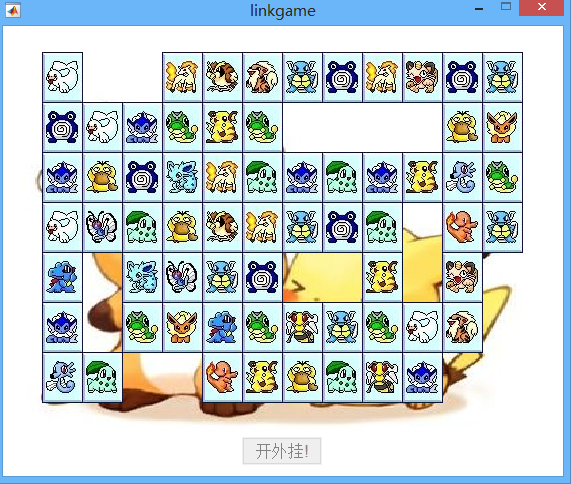
\includegraphics[width=0.7\textwidth]{match_adjacent}
                            \caption{测试\texttt{matchadj()}功能}
                        \end{figure}

                        \texttt{matchadj}函数工作正常。

                    \item \textbf{消去同一条边界上的相同块\texttt{matchborder}}:先定义\textbf{上边界},如图\ref{fig:upper_border}中的\textcolor{blue}{蓝色区域}。

                        \begin{figure}[H]
                            \centering
                            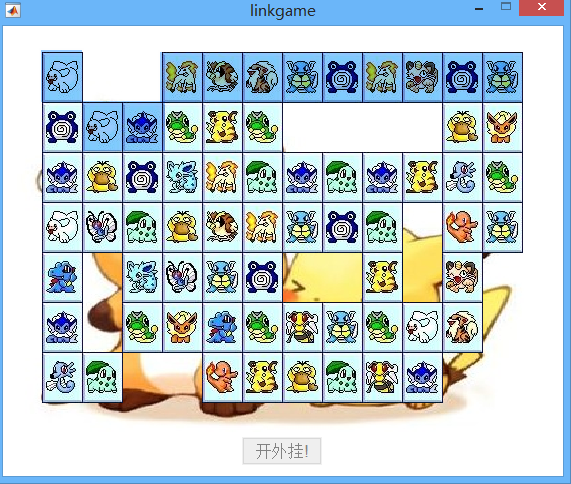
\includegraphics[width=0.7\textwidth]{upper_border}
                            \caption{定义上边界}
                            \label{fig:upper_border}
                        \end{figure}

                        显然,\textbf{上边界即每一列第一个非零元素};类似地可以定义其他边界。

                        容易证明,\textbf{在同一边界上的相同块必然可消去}。

                        与\texttt{matchadj}不同,由于消去过程会使边界发生变化,故必须不断循环直至边界保持不变。则实现\texttt{matchborder}函数如下:

                        \inputminted[firstline=79,lastline=135]{matlab}{../linkgame/omg.m}
                        \begingroup
                            \captionof{listing}{\texttt{omg.m(matchborder)}}
                        \endgroup

                        \begin{figure}[H]
                            \centering
                            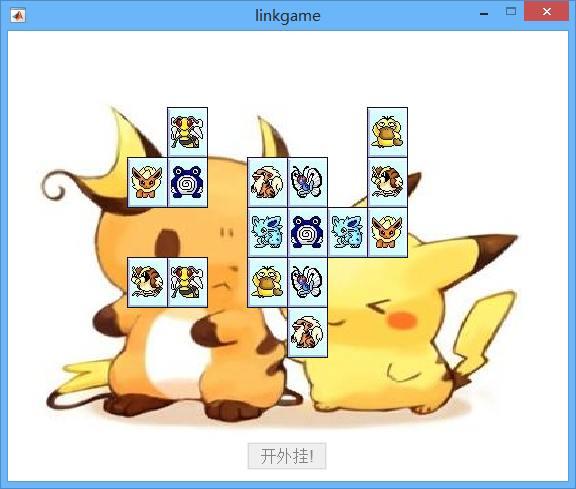
\includegraphics[width=0.7\textwidth]{match_border}
                            \caption{依次调用\texttt{matchadj}和\texttt{matchborder}后}
                            \label{fig:match_border}
                        \end{figure}

                        经过多次测试,发现\texttt{matchadj}与\texttt{matchborder}相结合的算法已经能消去游戏区域的\textbf{绝大多数块},甚至有时可\textbf{全部消去}。

                        \texttt{matchadj}的核心是\texttt{MATLAB}自带的\texttt{diff}函数,效率较高;

                        而\texttt{matchborder}通过\texttt{cumsum}以及\texttt{sum}函数巧妙获得各边界索引,再利用\texttt{unique}以及\texttt{find}等方法在边界内寻找相同的块,可以说十分高效。

                        既然高效的前两步已可以消去大多数块,那么对于剩余的块,不妨采取较暴力的算法解决。

                    \item \textbf{对于剩余的块按种类遍历尝试连接\texttt{matchrest}}:这里假设生成的连连看游戏是可以以任意消除顺序完全消除的(实践观测结果如此)。

                        \inputminted[firstline=138,lastline=164]{matlab}{../linkgame/omg.m}
                        \begingroup
                            \captionof{listing}{\texttt{omg.m(matchrest)}}
                        \endgroup

                        经过多次测试,均能顺利完成功能。

                \end{enumerate}

        \end{enumerate}

    % section 制作自己的连连看 (end)


\end{document}